\documentclass[a4paper, 12pt, master, utf8]{etf}

\usepackage[a4paper, margin=25mm]{geometry}
\usepackage{gentium} % font
\usepackage{enumitem}
\usepackage[linesnumbered, algoruled, longend]{algorithm2e} % za pseudo kod
\usepackage{rotating} % za sidetable

\addto\extrasserbianc{\def\bibname{Литература}\let\refname\bibname}
\SetAlgorithmName{Псеудо код}{псеудо код}{Листа псеудо кодова}
\SetInd{2mm}{3mm} % za pseudo kod razmak pre i posle
\newcommand*\rot{\rotatebox{90}} % za rotirane labele tabele

\author{Име Презиме}
\date{\today}
\title{Наслов}
\indeks{ГГГГ/ББББ}
\mentor{доц др. Марко Мишић}
\usepackage{array}
\newcolumntype{P}[1]{>{\centering\arraybackslash}p{#1}}
\usepackage{titlesec}
\usepackage{setspace}
\usepackage[flushleft]{threeparttable}
 
\titleformat{\chapter}[display]
  {\normalfont\bfseries}{}{0pt}{\Huge}

\begin{document}

\maketitle

\tableofcontents

\addtocontents{toc}{\protect\thispagestyle{empty}}
\pagenumbering{arabic}
\onehalfspacing
\newpage

\chapter{Увод}
\label{sec:1}

Овде иде увод.

\chapter{О проблему}
\label{sec:2}
У овом поглављу прво ће бити описан проблем који се решава, а затим ће се прећи на теоријске основе потребне за решавање тог проблема алгоритмима машинског учења...

\section{Формулација проблема}
\label{sec:21}
Проблем којим се овај рад бави је...

\begin{itemize}[noitemsep]
    \item  ставка,
    \item  ставка.
\end{itemize}

\section{Машинско учење}
\label{sec:22}
Надгледано учење је врста којом ће се овај рад бавити и оно се може по Шалеву-Шварцу \cite{anthony2009neural}...

\section{Неуронске мреже}
\label{sec:23}
На слици \ref{fig:neuron} графички је представљен један вештачкки неурона, као што је претходно описан.

\begin{figure}[h]
    \centering
    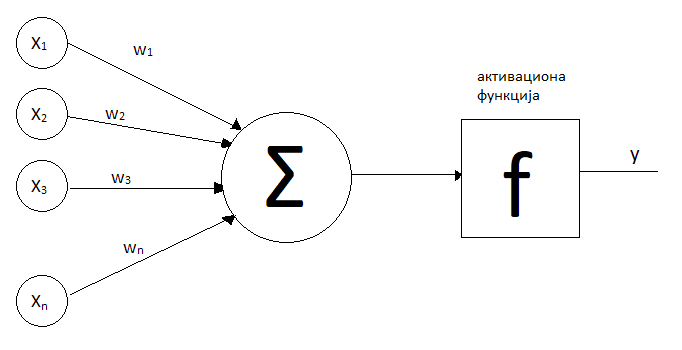
\includegraphics[width=.8\textwidth]{img/neuron.png}
    \caption{Вештачки неурон}
    \label{fig:neuron}
\end{figure}

\begin{figure}[h]
    \centering
    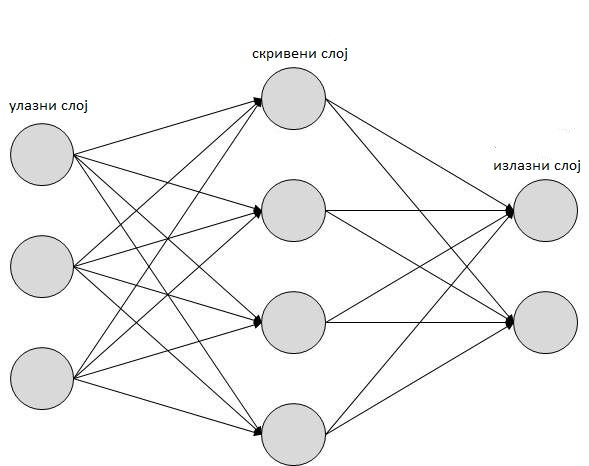
\includegraphics[width=.6\textwidth]{img/simple_net.jpg}
    \caption{Проста мрежа са пропагацијом унапред}
    \label{fig:simplenet}
\end{figure}

Пример једначине:
\begin{equation}
\label{2.1}
        \delta_j^l = \frac{\partial L}{\partial a_j^l}f^\prime(z_j^l),
\end{equation}

\subsection{Слојеви конволутивне неуронске мреже}
\label{sec:24}
Свака неуронска мрежа се састоји из неколико различитих типова слојева, и у наставку ће бити дати њихови описи.

\subsubsection{Слој конволуције}
Први, и основни, слој који конволутивна мрежа садржи је слој конволуције..

\chapter{Коришћене технологије}
\label{sec:3}
У овом поглављу ће бити описане коришћене технологије.

\begin{sidewaystable}[h]
    \centering
    \begin{tabular}{|l | P{2.5cm} | P{2.2cm} | P{2cm} | P{2.5cm} | P{2cm} | P{1.5cm} | P{3.5cm}|}
        \hline
            & Програмски језици & Докумен- тација & Ниво апстракције & Конволуционе мреже & Рекурентне мреже & Брзина извршавања & Подршка за више графичких процесора\\
        \hline
         TensorFlow & Python, Go, R, Java & +++ & + & +++ & ++ & + & ++ \\\hline
         MXNet & Python, R, Julia, Scala & ++ & ++ & ++ & + & +++ & +++ \\\hline
         Chainer & Python & + & + & ++ & ++ & ++ & +\\\hline
         Keras & Python, R & +++ & + & +++ & +++ & ++* & ++*\\\hline
         Pytorch & Python & ++ & + & +++ & ++ & +++ & ++\\\hline
    \end{tabular}
    \begin{tablenotes}
        \small
        \item Знак "+" представља интензитет тог поља у табели, где је минимум један, а максимум три.
        \item[*] (*) У зависности од коришћеног радног оквира у позадини
    \end{tablenotes}
    \caption{Преглед платформи за развој неуронских мрежа}
    \label{tab:platforms}
\end{sidewaystable}

\chapter{Опис решења}
\label{sec:4}

Решење проблема датог у делу \ref{sec:2}...

\begin{algorithm}
\label{alg1}
\DontPrintSemicolon
\For{$epoch \gets 1$ \KwTo $N$} {
    $train(data, model)$ \;
    $error_{epoch} = validate(data, model)$ \;
    \If{$error_{epoch - 1} - error_{epoch} > E$}{
        $model.save()$ \;
        $break$ \;
    }
}
 \caption{Главна петља}
\end{algorithm}

\chapter{Резултати и дискусија}
\label{sec:5}

У овом поглављу прво ће бити описан хардвер на коме су резултати добијени, затим софтверски стек (енг. \textit{software stack}) који је коришћен при тестирању како би се отклониле евентуалне системске зависности. Потом, биће представљени и резултати овог рада у виду више решења проблема, свако са својим каратеристикама. Финално, биће дискутоване разике између решења и њихова могућа побољшања. 

\section{Тест платформа}
\label{sec:51}

\section{Методологија тестирања}
\label{sec:52}

\section{Резултати и дискусија}
\label{sec:53}

Како би се приказала успешност неуронске мреже...

\begin{table}[h]
    \centering
    \begin{tabular}{l | c c}
    \hline
    време извршавања [s] & централни процесор & графички процесор\\
    \hline
        обучавање & 541.3  & 52.23\\
        валидација & 52.2 & 7.1
    \end{tabular}
    \caption{Однос времена извршавања на графичком и централном процесору}
    \label{tab:performanse}
\end{table}

\chapter{Закључак }
\label{sec:6}

Овај рад је увео проблем...

Једна занимљива идеја за будући рад би могла бити...

%\chapter{Литература}
%\label{sec:7}

% Predlažem upotrebu bibtex i kreiranje .bib fajlova, a da se podaci za njh skidaju sa Google Scholar i sličnih servisa
\bibliographystyle{ieeetr}
\bibliography{literatura.bib}
%\addcontentsline{toc}{chapter}{Литература}

% Alternativni način
%\begin{thebibliography}{10}
%\bibitem{Shalev-Shwartz:2014:UML:2621980}
%S. Shalev-Shwartz, S. Ben-David, \emph{Understanding MachineLearning}, Cambridge, 2016
%\end{thebibliography}

\end{document}